\section{Results and Discussion}
\label{sec:resultsanddiscussion}

Testing and analysis were conducted on the previously designed and implemented systems. The tests included Load Cell Sensor testing on the Robot and the Robot Balance System.

\begin{enumerate}[label=\Alph*.]

    \item Characterization Testing on Each Load Cell Sensor
    \label{subsec:results-discussion-characterization}

        \hspace*{1em} Calibration tests for the load cell sensors were conducted using five reference mass weights (50g, 100g, 200g, 500g, and 1000g) to determine the gradient coefficient and tare weight constant. The load cells were connected in two groups: Load Cell 1 and 4, and Load Cell 2 and 3.

        \begin{table}[h]
            \centering
            \caption{First Load Cell Characterization Results}
            \begin{tabular}{|c|c|c|}
                \hline
                \textbf{Actual Weight (g)} & \textbf{Load Cell 1 Reading (g)} & \textbf{Error (g)} \\
                \hline
                50    & 50    & 0   \\
                100   & 101   & 1   \\
                200   & 202   & 2   \\
                500   & 505   & 5   \\
                1000  & 1004  & 4   \\
                \hline
            \end{tabular}
            \label{tab:Calibration_Load_Cell_1}
        \end{table}

        \begin{table}[h]
            \centering
            \caption{Second Load Cell Characterization Results}
            \begin{tabular}{|c|c|c|}
                \hline
                \textbf{Actual Weight (g)} & \textbf{Load Cell 2 Reading (g)} & \textbf{Error (g)} \\
                \hline
                50        & 50        & 0   \\
                100       & 100       & 0   \\
                200       & 200       & 0   \\
                500       & 500       & 0   \\
                1000      & 994       & 6   \\           
                \hline
        \end{tabular}
        \label{tab:Calibration_Load_Cell_2}
        \end{table}

        \begin{table}[h]
            \centering
            \caption{Third Load Cell Characterization Results}
            \begin{tabular}{|c|c|c|}
                \hline
                \textbf{Actual Weight (g)} & \textbf{Load Cell 3 Reading (g)} & \textbf{Error (g)} \\
                \hline
                50        & 50        & 0    \\    
                100       & 103       & 3    \\    
                200       & 203       & 3    \\    
                500       & 494       & 6    \\    
                1000      & 981       & 19   \\               
                \hline
        \end{tabular}
        \label{tab:Calibration_Load_Cell_3}
        \end{table}

        \begin{table}[h]
            \centering
            \caption{Fourth Load Cell Characterization Results}
            \begin{tabular}{|c|c|c|}
                \hline
                \textbf{Actual Weight (g)} & \textbf{Load Cell 4 Reading (g)} & \textbf{Error (g)} \\
                \hline
                50        & 50        & 0   \\     
                100       & 97        & 3   \\     
                200       & 204       & 4   \\     
                500       & 500       & 0   \\     
                1000      & 1003      & 3   \\                
                \hline
        \end{tabular}
        \label{tab:Calibration_Load_Cell_4}
        \end{table}
    
        
        \hspace*{1em} The digital readings from the load cells were converted into actual mass using calibration equations, and errors were measured by comparing the results with the actual masses. The measurement results showed errors ranging from 0 to 20 grams. Although not entirely linear, the calibration equations used were sufficiently accurate with an error tolerance of 5%.

    \item Pressure Testing on Foot Soles
    \label{subsec:results-discussion-pressure}

        \hspace*{1em} This test was conducted to obtain pressure data generated by the right and left feet when equally loaded. The pressure data generated by the right and left feet can be seen in Table \ref{tab:left_foot_weight_measurement} and Table \ref{tab:right_foot_weight_measurement}.

        \begin{table}[h!]
            \centering
            \caption{Pressure Reading Table for the Left Foot}
            \begin{tabular}{|c|c|c|}
                \hline
                \textbf{Actual Weight (g)} & \textbf{Reading (g)} & \textbf{Error (g)} \\
                \hline
                50    & 52    & 2   \\
                100   & 110   & 10  \\
                200   & 220   & 20  \\
                300   & 304   & 4   \\
                500   & 512   & 12  \\
                700   & 701   & 1   \\
                1000  & 1050  & 50  \\
                1300  & 1325  & 25  \\
                1500  & 1512  & 12  \\
                1800  & 1788  & 12  \\
                \hline
                \textbf{Average Error (g)} & \multicolumn{2}{c|}{\textbf{14.8}} \\
                \hline
            \end{tabular}
            \label{tab:left_foot_weight_measurement}
        \end{table}

        \begin{table}[h!]
            \centering
            \caption{Pressure Reading Table for the Right Foot}
            \begin{tabular}{|c|c|c|}
                \hline
                \textbf{Actual Weight (g)} & \textbf{Reading (g)} & \textbf{Error (g)} \\
                \hline
                50    & 46    & 4    \\
                100   & 98    & 2    \\
                200   & 215   & 15   \\
                300   & 325   & 25   \\
                500   & 505   & 5    \\
                700   & 722   & 22   \\
                1000  & 1025  & 25   \\
                1300  & 1347  & 47   \\
                1500  & 1500  & 0    \\
                1800  & 1819  & 19   \\
                \hline
                \textbf{Average Error (g)} & \multicolumn{2}{c|}{\textbf{16.4}} \\
                \hline
            \end{tabular}
            \label{tab:right_foot_weight_measurement}
        \end{table}

        \hspace*{1em} Based on the test results, the average error produced by the left foot is 14.8 grams, and the right foot is 16.4 grams.

    \item Center of Pressure Testing on the Robot
    \label{subsec:results-discussion-cop}

        \hspace*{1em} This test was conducted by moving the robot in a walking pattern and taking input data from the pressure sensors at 50 ms intervals. The purpose of this test is to obtain center of pressure data when the robot is performing walking movements and to observe how the center of pressure changes during movement. The Center of Pressure Testing Results on the Robot can be seen in Figure \ref{fig:robot_cop}.

        \begin{figure}[h]
            \centering
            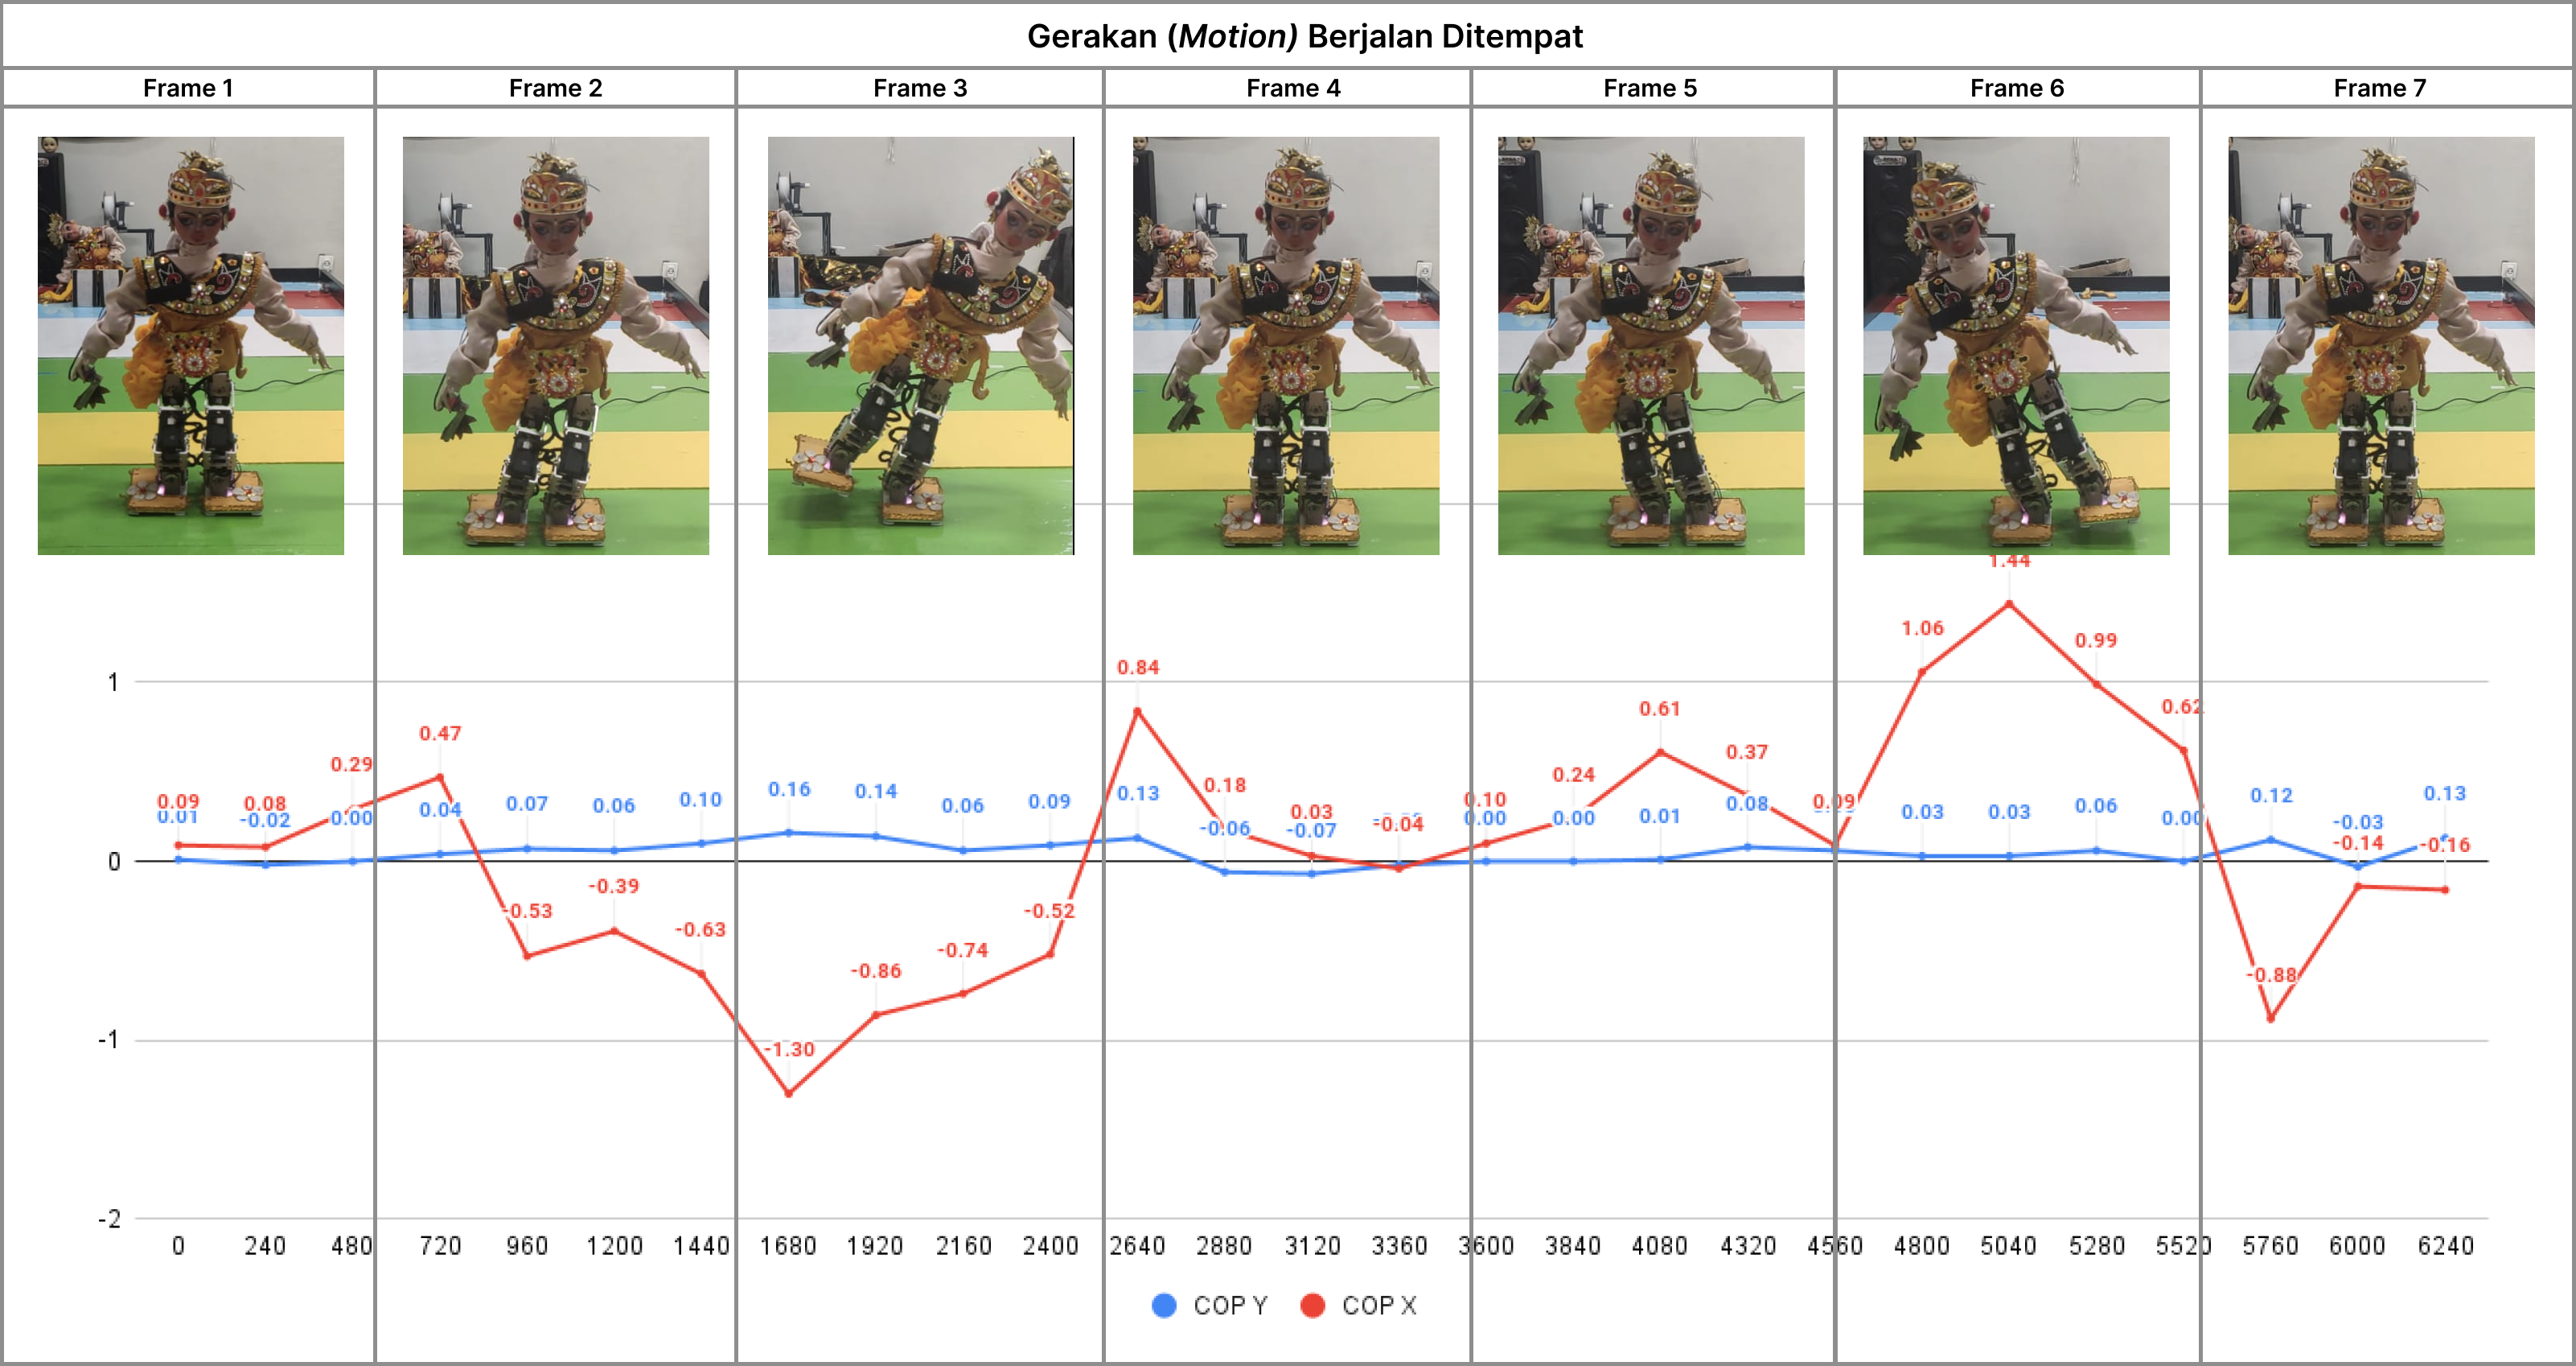
\includegraphics[width=0.45\textwidth]{gambar/motion_berjalan.png}
            \caption{Center of Pressure Graph When the Robot Walks in Place}
            \label{fig:robot_cop}
        \end{figure}

        \hspace*{1em} The test results showed that the center of pressure changes dynamically while the robot performs walking movements. When the robot lifts its right leg, the center of pressure shifts to the left leg, and the center of pressure value on the X-axis has a maximum value of 1.44. Conversely, when the robot lifts its left leg, the center of pressure shifts to the right leg, and the center of pressure value on the X-axis has a minimum value of -1.3. On the Y-axis, the center of pressure value ranges from 0.16 to -0.06, indicating that the center of pressure is in the middle of the foot sole.

    \item PID Control System Testing
    \label{subsec:results-discussion-pid}

        \hspace*{1em} This test will compare the effect of the \(K_p\) parameter on the PID control system performance. The test is conducted by measuring the Root Mean Square (RMS) and the test results on lifting the right and left legs.

        \begin{table}[h]
            \centering
            \caption{Root Mean Square (RMS) in the Effect of P Parameter Testing}
            \begin{tabular}{|c|c|}
            \hline
            \textbf{PID} & \textbf{RMS Error} \\
            \hline
            $K_p = 0.00$ & 0.7598 \\
            $K_p = 0.05$ & 0.7690 \\
            $K_p = 0.10$ & 0.7779 \\
            $K_p = 0.15$ & 0.8145 \\
            $K_p = 0.20$ & 0.8870 \\
            $K_p = 0.25$ & 0.8801 \\
            \hline
            \end{tabular}
            \label{tab:rms_p}
        \end{table}

        \begin{table}[h]
            \centering
            \caption{Test Results of the Effect of P Parameter on PID Controller, Right Leg Lifting Movement}
            \begin{tabular}{|c|c|c|c|}
                \hline
                \textbf{PID} & \textbf{Fall} & \textbf{Not Fall} & \textbf{Success} \\
                \hline
                $K_p = 0.00$ & 6 & 0 & 0   \% \\
                $K_p = 0.05$ & 6 & 0 & 0   \% \\
                $K_p = 0.10$ & 0 & 6 & 100 \% \\
                $K_p = 0.15$ & 1 & 5 & 83  \% \\
                $K_p = 0.20$ & 0 & 6 & 100 \% \\
                $K_p = 0.25$ & 2 & 4 & 66  \% \\            
                \hline
            \end{tabular}
            \label{tab:testing_p_right}
        \end{table}

        \begin{table}[h]
            \centering
            \caption{Test Results of the Effect of P Parameter on PID Controller, Left Leg Lifting Movement}
            \begin{tabular}{|c|c|c|c|}
                \hline
                \textbf{PID} & \textbf{Fall} & \textbf{Not Fall} & \textbf{Success} \\
                \hline
                $K_p = 0.00$ & 6 & 0 & 0   \% \\
                $K_p = 0.05$ & 6 & 0 & 0   \% \\
                $K_p = 0.10$ & 0 & 6 & 100 \% \\
                $K_p = 0.15$ & 1 & 5 & 83  \% \\
                $K_p = 0.20$ & 1 & 5 & 83  \% \\
                $K_p = 0.25$ & 0 & 6 & 100 \% \\            
                \hline
            \end{tabular}
            \label{tab:testing_p_left}
        \end{table}

        \hspace*{1em} From the test results presented in the tables, the optimal value of the \(K_p\) parameter that allows the robot to maintain balance well ranges from 0.10 to 0.20. At \(K_p\) = 0.00 and \(K_p\) = 0.05, all tests failed with the robot always falling, indicating that the PID control is ineffective at those values. Conversely, the \(K_p\) value of 0.10 shows the best performance with a 100\% success rate in maintaining the robot's balance during right and left leg lifting movements on a 3-degree slope.

        \hspace*{1em} Then, from the Root Mean Square (RMS) results presented in Table \ref{tab:rms_p}, it can be seen that the smallest RMS value is obtained at \(K_p\) = 0.10, indicating the least inaccuracy in the system at this value.

\end{enumerate}
